\def\year{2016}\relax
%File: formatting-instruction.tex
\documentclass[letterpaper]{article}
\usepackage{aaai16}
\usepackage{times}
\usepackage{helvet}
\usepackage{courier}
\usepackage{graphicx}
\usepackage{booktabs} % for pretty table rules
\usepackage{hyperref}
\usepackage[T1]{fontenc}

\frenchspacing
\setlength{\pdfpagewidth}{8.5in}
\setlength{\pdfpageheight}{11in}
\pdfinfo{
/Title Wikidata Human Gender Index: An Open Dataset with Perspectives on Times, Space, and Occupation
/Author Max Klein, Harsh Gupta, Vivek Rai, Haiyi Zhu}
\setcounter{secnumdepth}{0}  
 \begin{document}
% The file aaai.sty is the style file for AAAI Press 
% proceedings, working notes, and technical reports.
%
\title{Wikidata Human Gender Index: An Open Dataset with Perspectives on Times, Space, and Occupation}

\author{AUTHORS BLINDED}
    
\maketitle
\begin{abstract}
AAAI creates proceedings, working notes, and technical reports directly from electronic source furnished by the authors. To ensure that all papers in the publication have a uniform appearance, authors must adhere to the following instructions. 
\end{abstract}


\section{Introduction}
Wikipedia has a gender gap. Wikidata offers new opportunities. \cite{wikidata-release}
Measuring the gender gap in content solves two problems. One is, what gets measured gets fixed. Furthermore, the scope of Wikidata gives us an unprecedented look at gender through time, space, and occupation which has practical applications for data mashups. 

Landscape of ways in which Wikipedia shows bias, and Landscape of biases. \cite{Wagner}. And has shown to be true particularly for the Wikipedia content gap \cite{carlosnotebook}.

We introduce a dataset called Wikidata Human Gender Index (WHGI), which is.

It is longitudinal, and we present summary statistics from our snapshotting. Our first observation is from September 17th 2014, and latest is January 3rd 2016. Although our dataset is updated weekly following the official Wikidata data dumps \footnote{•}.

WHGI is not a not entirely Wikipedia navel-gazing, we present 3 validation measures that show that it is increasingly representing the real world. This means that albeit with caveats and huge biases, if the data is to believed, affords us an unprecedented look at gender representation on a time and geographic scale not possible before.

The WHGI is meant for re-use, and we present some of the potential applications 

\section{Dataset Details}

\begin{figure}
\label{fig:screenshot}
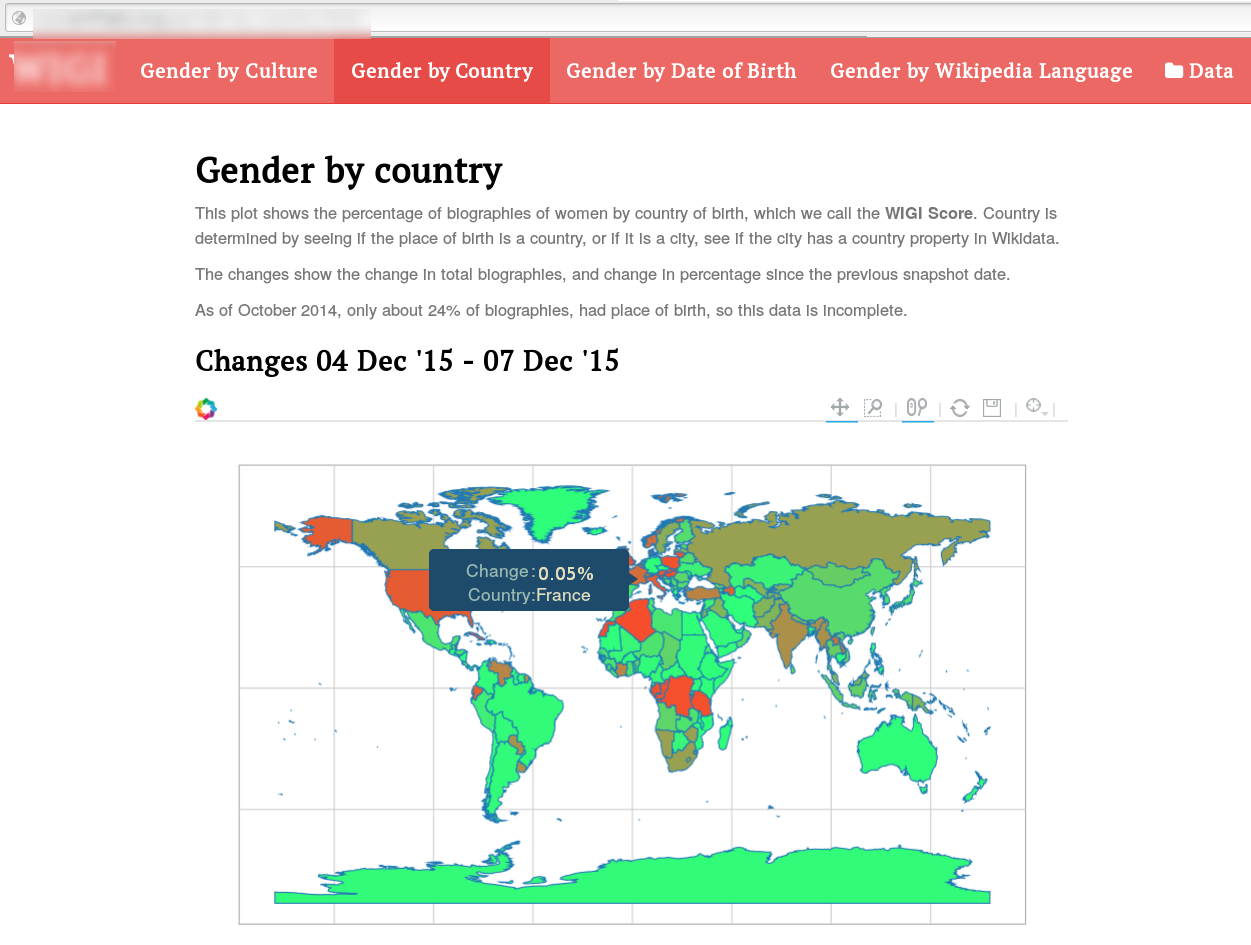
\includegraphics[scale=0.2]{figures/website_screenshot.png} 
\caption{Screenshot of WEBSITE BLINDED displaying the gender by culture plot.}
\end{figure}

Our dataset is available for free under the CC0 license online at  \url{WEBSITE BLINDED} . Here a visualization demonstration of our data lives, and direct downloads, from the \url{WEBSITE BLINDED/} folder. 	This folder contains the CSV-formatted, weekly captured \textit{snapshots} of gender-related data from Wikidata. Each snapshot contains an unaggregated one-row-per-human complete view of the data, \textit{re-indexed} ``property"-specific file, aggregated by tempo, spatial, and other properties, and weekly changes between the property indexes.

\subsection{Processing}
Each week, just after the release of Wikidata's official weekly data dump, we download a copy of the dump and process it in the following way. Using the Wikidtata Toolkit \cite{kroetsch} the entire database is subsetted to only those items which have the property \textit{instance of} with value \textit{human} - or ``P31:Q5" in Wikidata terms. For each human item we find the values of \textit{gender}, \textit{date of birth}, \textit{date of death}, \textit{place of birth}, \textit{citizenship}, \textit{ethnic group}, \textit{field of work}, and \textit{occupation}. These correspond to Wikidata properties P21, P569, P570, P19, P27, P172, P101, and P106 respectively.  In every snapshot folder this intermediate step is saved as ``gender-index-data-\{snapshot data\}.csv", it records one Wikidata item per row, and it's columns are the value of each property.
 
For each of the recorded properties we then re-index the dataset aggregated on that property, but disaggregated by gender. So for instance, the date of birth index has one row per year unique year found as a date of birth, and one column per gender represented in Wikidata. For example the in the January 3\textsuperscript{rd} 2016 snapshot, the first row the date of birth index reads that for the year 4203 BCE Wikidata records two men, and no other genders as having this date of birth. Additionally there are indexes, that make use of the Wikipedia languages in which a human is represented - \textit{sitelinks}, and geographic aggregations of citizenship, place of birth and ethnic group into properties called \textit{culture}, and \textit{worldmap}. Inside every snapshot folder there exists a subfolder titled ``property-indexes" containing 11 ``re-indexes" of the snapshot - one per property dimension.
 
 The third item in every snapshot folder is titled ``changes-since- \{previous snapshot date\}, and contains computed differences between this snapshot and the last. This feature allows inspection of the movements of the past week. There is one ``changes-since" file for each property file. Using the date of birth example again, the changes since file will show which genders were added - or subtracted - for each year, in the course of the week.

Examples of how to process the CSVs using both \textit{python-pandas} and \textit{R} can be found in our github repository \footnote{\url{WEBSITE BLINDED}}. 

As a demonstration the website displays 4 interactive visualizations of the dataset. Figure \ref{fig:screenshot} shows the \textit{gender-by-country} visualization, which shows the female ratio of humans by place of birth and citizenship combined. The visualizations show \textit{gender-by-culture}, where culture is a further aggregation of countries, \textit{gender-by-date-of-birth-and-death} and \textit{gender-by-Wikipedia-language}.

Additionally there are two special folders in our root directory which we offer for convenience,  titled \textit{newest} and \textit{newest-changes}, which will always link to the most recent snapshot, and the changes between the two most recent snapshots (week to week), respectively. This makes it easy to always access the freshest data.

In order to faithfully represent Wikidata, the value of each property is actually a list, since Wikidata allows there to potentially be many competing values for a property. (We store the list, inside the comma-separated sheet, as | ``pipe"-separated values.)  Also note, for faithfulness there is virtually no data-cleaning done, as the point of our project is to display information as faithfully as possible. Our dataset is meant to be used to uncover potential biases in Wikidata and the world at large, and we feel that any cleaning process would introduce further biases.

\section{Dataset Statistics}
We now turn to look at simple statistics of our dataset, specifically with regard to how it has changed over time. Our first snapshot was on September 17\textsuperscript{th} 2014, and the latest analysed here is January 3\textsuperscript{rd} 2016. Since automation of snapshotting was not completed until June 28th 2015, there is unfortunately a window missing from October 2014 to June 2015. 

\subsection{Data Quality}
Let us first query the size of the dataset. Total humans in Wikidata increased from 5,869,606 to 6,999,542, and shows linear, unconstrained growth (see Figure \ref{fig:totalhumans}).
\begin{figure}
\label{fig:totalhumans}
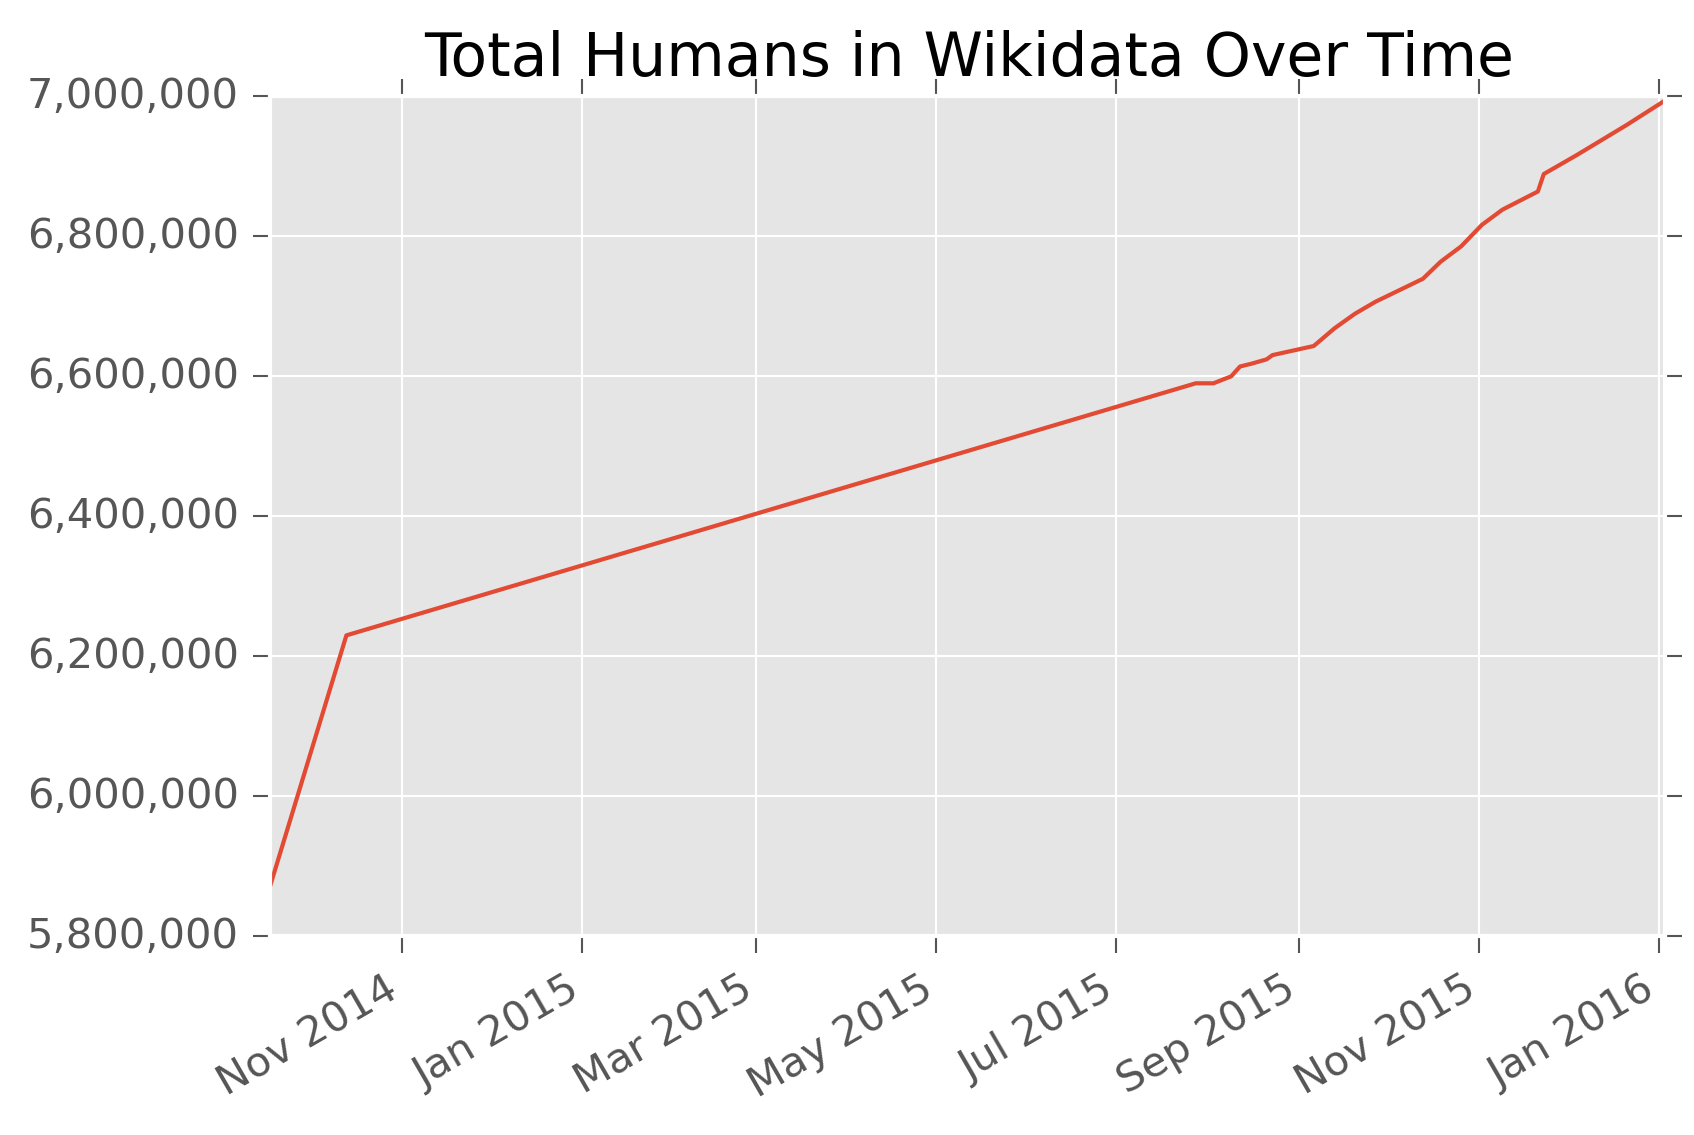
\includegraphics[scale=0.6]{figures/totalhumans.png} 
\caption{Total number of humans found in Wikidata at each snapshot period.}
\end{figure}

We should also be curious to the data quality of the increasing humans. One way to think about this is about the how much data is accompanying these human entries. We looked at the properties citizenship, place of birth, and ethnic group which will help us best geographically place a human. Another mark of quality is whether a human in Wikidata has an entry in a Wikipedia - a ``sitelink" in Wikidata vocabulary. Figure \ref{fig:accompanying} shows the rate of accompanying properties, at the earliest and latest snapshots from 2014 and 2016 respectively. The statistics show that data quality has been increasing almost uniformly over time. The number of humans with \textit{gender} data increased by over 1\%, closer to complete coverage. In the time domain \textit{date of birth} and \textit{date of death}coverage increased by 14\% and 7\%. Likewise \textit{citizenship} data increased by 15\% , \textit{place of birth} by 6\% , and \textit{ethnic group} almost doubled (see Table \ref{table:accompanying}). Field of work, and occupation data was not included in our dataset until late, so their growth, while increasing is not precisely comparable.

Curiously the rate of humans having sitelinks decreased slightly, but this is important as well A Wikidata human without a Wikipedia article is know as a ``structural item"; for instance a member of royalty without a Wikipedia article but is a needed to make a family tree complete. With the view that a structural item is an artefact from humans paying attention to Wikidata's structure, the decrease in sitelinked humans can also be seen as a rise in data quality.


\begin{table}
\caption{Change in rates of human-accompanying properties}
\begin{tabular}{lrr}
\toprule
{} &  2014-09-17 &  2016-01-03 \\
\midrule
gender               &       95.3\% &       96.5\% \\
date of birth        &       57.6\% &       71.7\% \\
date of death        &       28.6\% &       36.1\% \\
citizenship          &       42.8\% &       58.2\% \\
place of birth       &       24.0\% &       30.5\% \\
ethnic group         &        0.3\% &        0.6\% \\
field of work        &        n/a &        0.3\% \\
occupation           &        n/a &       58.7\% \\
at least 1 site link &       99.6\% &       98.1\% \\
\bottomrule
\end{tabular}
\label{table:accompanying}
\end{table}

\begin{figure}
\label{fig:accompanying}
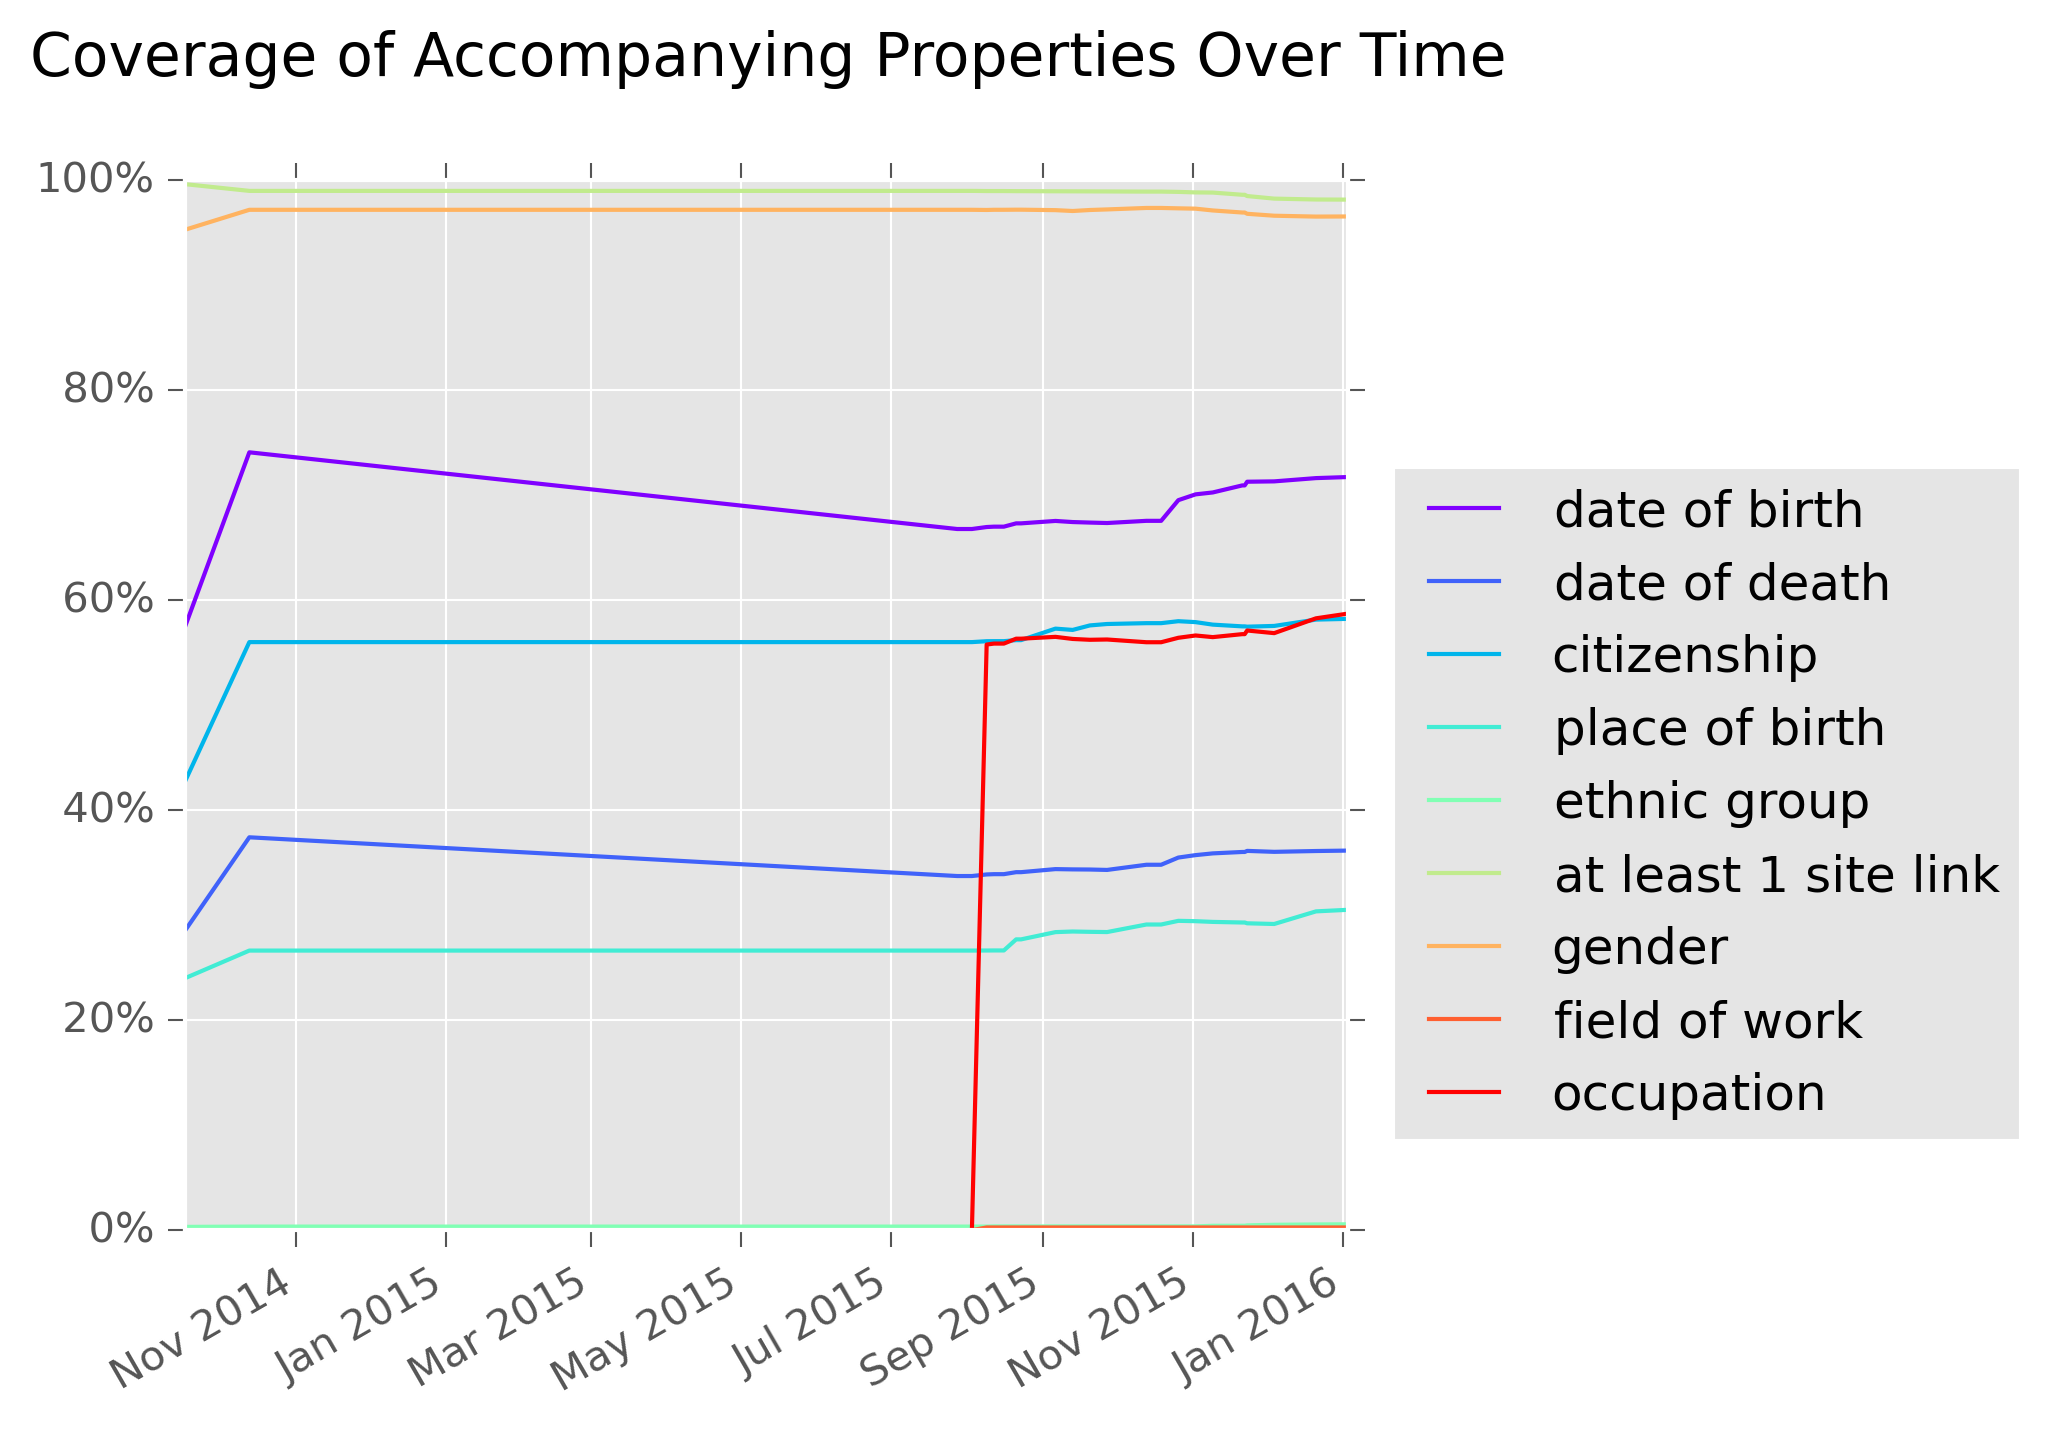
\includegraphics[scale=0.5]{figures/additionalprops.png} 
\caption{Trend of human-accompanying properties by snapshot.}
\end{figure}

An important factor to note, as mentioned, is that our dataset does is not \textit{cleaned} to fit any model. In fact the ``gender" property in Wikidata is actually labelled in English ``sex or gender" (no distinction), and not limited to any value. Over our time snapshotting we found 36 values used for ``sex or gender", including ``male" and ``female", but extending to nonbinary genders ``transgender female", ``intersex", ``fa'afafine", ``transgender", ``Gender fluid",  ``genderqueer", ``kathoey", and ``queer". At times the other categories of information is recorded here - perhaps erroneously - such as ``gay", or ``homosexuality". And even what seem to be mistakes are left in such as one-offs of ``Solanum tuberosum", ``Messi", or ``sociologist".

\subsection{Simple Metrics}
As further motivation for how the dataset can be used, we present some simple metrics which would be of interest to Wikimedian communities. Focusing on one of our motivations, monitoring the trend of gender representation, we inspect the rate at which women are recorded in Wikidata. Figure \ref{fig:frb} shows the ratio of ``female" recorded humans versus all gendered biographies. Similarly to total biographies this measure is rising at a fairly linear rate of approximately 0.5\% per year. The final months on record show a slight decline which warrants further investigation. In fact being able to measure at this temporal level is precisely one of the points of having such a live-updating measure - to be able to detect trends as they happen, and perhaps relate them to community issues. 

\begin{figure}
\label{fig:frb}
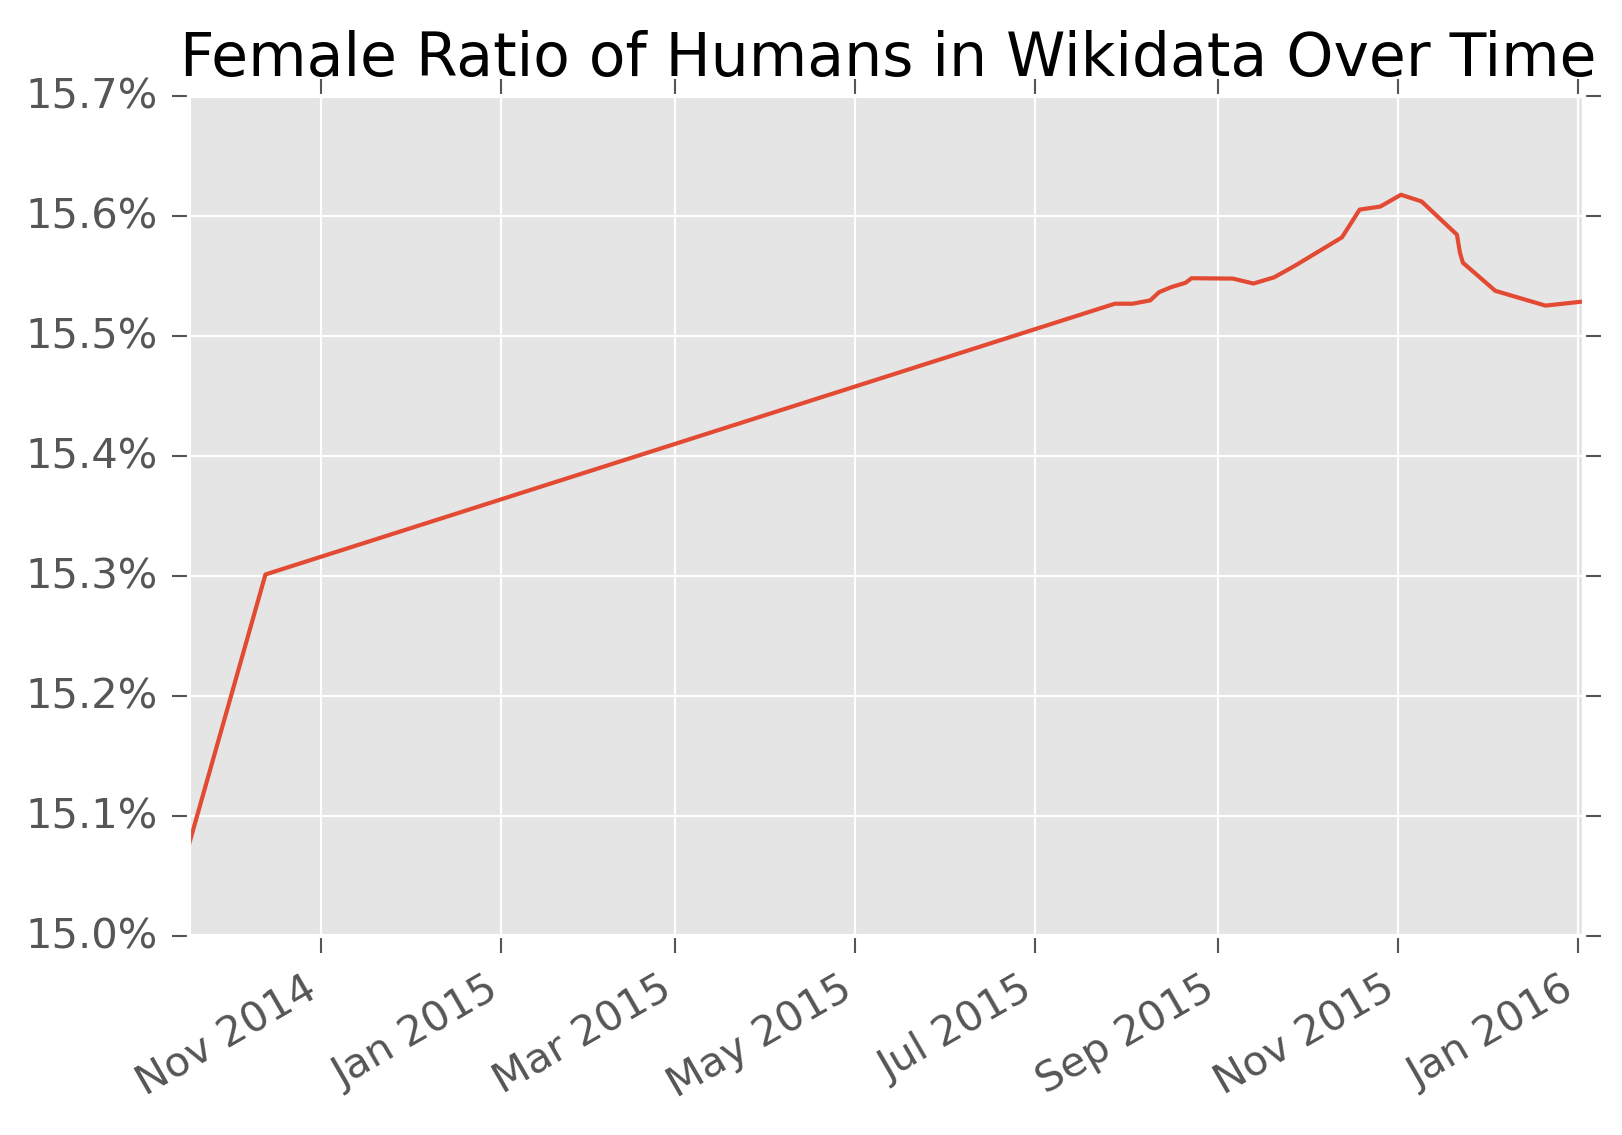
\includegraphics[scale=0.6]{figures/frbwikidata.png} 
\caption{Trend of human-accompanying properties by snapshot.}
\end{figure}

Another way in which Wikimedians can use the data is to look at trends specific to Wikipedia languages. It is easy to use the data to compile a top-10 list of Wikipedias whose female ratio of humans increased the most, see Table \ref{table:top10}. This measure does not explain whether women's representation in those languages increased because because editors took longer to record women's gender in Wikidata and were catching up in the observed period, or that these languages became more women-focused over the snapshotting period. Such forensics is possible with this dataset though.

\begin{table}
\caption{Top 10 Wikis by increase in female ratio of humans from October 2014 to January 2016}
\label{table:top10}
\begin{tabular}{p{2cm}p{2cm}}
\toprule
{Wiki} &     Increase in female ratio of humans  \\
\midrule
Lithuanian      & 5.31\% \\
Japanese     & 4.76\% \\
Estonian      & 4.58\% \\
Slovenian      & 2.19\% \\
Tagalog      & 1.63\% \\
Korean      & 1.38\% \\
Finnish      & 1.33\% \\
Wikimedia Commons & 1.20\% \\
Farsi      & 1.17\% \\
Hebrew      & 1.17\% \\
\bottomrule
\end{tabular}


\end{table}

\section{Validation}
In order to gain an idea about how well WHGI reflects the real world, we validated out data by comparing it against 3 exogenous datasets. We correlated the WHGI date of birth frequency versus historical world population trends; WHGI gender by country versus external by-country gender-disparity indexes; and WHGI occupation by gender versus United States Bureau of Labor Statistics occupation gender.

\subsection{World Population}

\subsection{Exogenous Gender-Disparities Indices}

 \begin{table}
\caption{WHGI-country correlation to external indices. Correlation is the Spearman $\rho$, and signficances are $ ^*p\leq 0.05 $, $ ^{**}p\leq 0.01$.}
\label{table:scores}
\begin{tabular}{lrrrr}
\toprule
snapshot &  GEI &  SIGI &  GGGI &  GDI  \\
\midrule
2014-09-17 &  0.417** &       0.338** &          0.310* &         0.278**  \\
2016-01-03 &  0.457** &       0.402** &          0.386** &         0.299**  \\
\bottomrule
\end{tabular}
\end{table}

WHGI is inspired in part by the rich landscape of gender disparity indices, such as The Gender Development Index (\textbf{GDI}) from the United Nations Development program. This type of index ranks countries by their gender equality. If we aggregate WHGI by place of birth and citizenship, and look at the female ratio of humans, we too have a country-by-gender equality measure.  We correlated the country rankings of this WHGI with 4 popular exogenous indices to see how well Wikidata reflects real world gender disparities. 

The 4 exogenous indices we used were: The United Nations' Gender Development Index (\textbf{GDI})  \footnote{\url{http://hdr.undp.org/en/content/gender-development-index-gdi}},  Social Watch's Gender Equity Index (\textbf{GEI}) \footnote{\url{http://www.socialwatch.org/node/14366}},  the Global Gender Gap Index (\textbf{GGGI}) \footnote{\url{http://reports.weforum.org/global-gender-gap-report-2014/}}, and the Social Institutions and Gender Index (\textbf{SIGI}) \footnote{\url{http://www.genderindex.org/ranking}}. 

Additionally we conducted a calibration step, to find the date of birth threshold which maximized our correlations. In each case the maximizing threshold was found to be between 1900 and 1910. We interpreted as a good sign firstly because the exogenous indices are measures of recent history, and secondly because of the stability in the way that WHGI relates exogenous indices.

Table \ref{table:scores} shows the the correlations with each index, all of which were significant and ranged from 0.278 to 0.457. The ways in which WHGI correlates more to indices that focus on positions of power than indices which focus on health measures, show that Wikipedias' notability policies are are similarly biased [AUTHOR BLINDED].  Affirmingly, when looking at this information through a snapshotting lens, the correlation with every index is increasing over time. That is, the gender disparities found in WHGI by country are looking more like the real world gender disparities. 


\subsection{Bureau of Labor Statistics}


 In context with the fact that data quality is rising, this can be taken to mean that as Wikidata becomes more complete it is modelling the real world more. 

\section{Potential Applications}
Though we believe in what Open Knowledge Foundation founder Rufus Pollock once said ``The best thing to do with your data will be thought of by someone else. " we still present a few ideas to stoke creativity. Since the data arises from Wikipedia, its introspective uses are many, but we also propose uses that are completely unrelated to the Wiki-universe. 

Wikimedian communities can use WHGI to measure their editorial and content focus. With the temporal nature of the snapshotting, applications could be built to detect spikes in creation or deletion of humans. This could be useful to measure the effectiveness of editathons, and other planned editing. However such a tool could also alert to the presence of unplanned activity, good or bad, which effects the macro-level gender of Wikipedia and Wikidata.

Divorced from Wikipedia entirely, a historian could use the data to determine the gender-disparity levels of a specific place and time. Typically to quantify the gender climate one would rely on the indexes like those mentioned in the Exogenous Indices section. However these indices, are limited to discussing recent history. With large caveats about accuracy and editor bias, our validation showed that our data is in touch with the real world to some degree. With this dataset we can quantify a type of gender-disparity of medieval France, ancient Greece, or Ming dynasty China. Generally WHGI is useful in all the same ways that exogenous indices are used, only with a larger timespan. That is certainly a novel approach not possible before Wikidata.

Yet another new avenue this dataset opens is in the gender-disparity of a language. There are several theories about how language affects gender \cite{} \cite{}. A linguistic could use WHGI aggregated by language to quantify the gendered-ness of a language. Furthermore with the date of birth and death information, that linguistic could see how languages have focus on gender differently over time, potentially backing up a theory of language that comes from their native methods. 

\section{Conclusion}
We made it because. It is easy to use, it can show some things about Wikipedia. Its also a validated measure of the real world. There are lots of potential ways in which it could be used.	


\section{ Acknowledgments}
We are especially grateful to the Wikimedia Foundation for funding us through an Individual Engagement Grant.

\bibliographystyle{aaai}
\bibliography{sample}

\end{document}
